\subsection{Estimator design}
\label{estimator}

Using an estimator, the states of the system can be reconstructed from the available voltage measurement on the output and the input of the system. While designing an observer (estimator), the main task is to estimate state $\mathbf{x}[k]$ from input and output sequences $y[k], y[k-1],..., u[k], u[k-1]$ .
During the real-life measurements, the estimates are provided by the same model placed parallel to the measured system. Even though, the system for the estimation is driven by the same input, in practice, uncertainties are expected. Which means that even if the initial state of the model is set equal to the initial state of the plant, in practice, without feedback the state estimate would diverge from the true state. The solution to this is to use the output measurements and make a comparison between that and the predicted output data. For that reason the difference can be used to modify the state estimate in such a way that it converges to the true state vector. The algorithm is illustrated in \figref{fig:algorithm} for the whole system.

\begin{figure}[H]
\centering

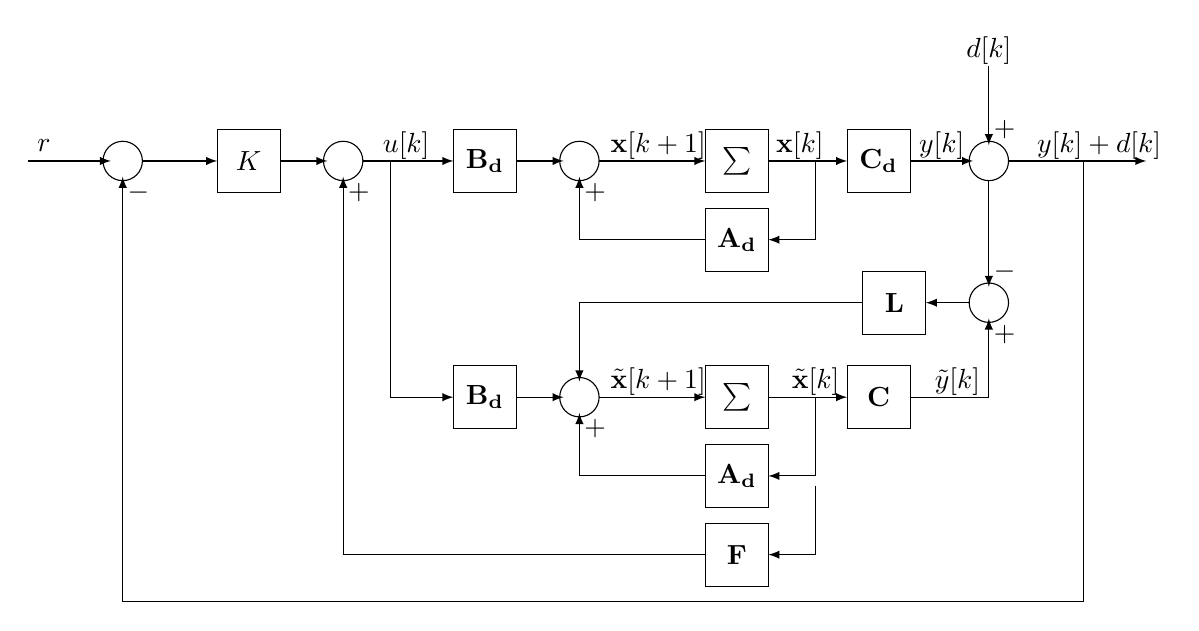
\begin{tikzpicture}
\node at (2.4,3.4) {\normalsize{$\mathbf{C_d}$}};
 \draw [-latex] (3.8,3.4) ellipse (0.25 and 0.25);
\draw [-latex] (2,3.8) rectangle (2.8,3);
\draw [-latex](2.8,3.4) -- (3.6,3.4);
\draw [-latex](3.8,4.6) -- (3.8,3.6);
\node at (3.2,3.6) {$y[k]$};
\node at (3.8,4.8) {$d[k]$};
\node at (0.6,3.4) {$\sum$};
\draw [-latex] (0.2,3.8) rectangle (1,3);
\draw [-latex](1,3.4) -- (2,3.4);
\node at (1.4,3.6) {$\mathbf{x}[k]$};
 \draw [-latex] (-1.4,3.4) ellipse (0.25 and 0.25);
\draw [-latex](-1.15,3.4) -- (0.2,3.4);
\node at (-0.4,3.6) {$\mathbf{x}[k+1]$};
\node at (0.6,2.4) {\normalsize{$\mathbf{A_d}$}};
\draw [-latex] (0.2,2.8) rectangle (1,2);
\draw [-latex](1.6,3.4) -- (1.6,2.4) -- (1,2.4);
\draw [-latex](0.2,2.4) -- (-1.4,2.4) -- (-1.4,3.2);
\node at (-2.6,3.4) {\normalsize{$\mathbf{B_d}$}};
\draw [-latex] (-3,3.8) rectangle (-2.2,3);
\draw [-latex](-2.2,3.4) -- (-1.6,3.4);
\draw [-latex] (-4.4,3.4) ellipse (0.25 and 0.25);
\draw [-latex](-4.15,3.4) -- (-3,3.4);
\node at (-3.6,3.6) {$u[k]$};
\node at (-5.6,3.4) {\normalsize{$K$}};
\draw [-latex] (-6,3.8) rectangle (-5.2,3);
\draw [-latex](-5.2,3.4) -- (-4.6,3.4);
\draw [-latex](4.05,3.4) -- (5.8,3.4);
\node at (5.2,3.6) {$y[k]+d[k]$};
\draw [-latex] (3.8,1.6) ellipse (0.25 and 0.25);
\draw [-latex](3.8,3.15) -- (3.8,1.8);
\node at (4,2) {$-$};
\node at (4,3.8) {$+$};
\node at (2.4,0.4) {\normalsize{$\mathbf{C}$}};
\draw [-latex] (2,0.8) rectangle (2.8,0);
\draw [-latex](2.8,0.4) -- (3.8,0.4) -- (3.8,1.4);
\node at (4,1.2) {$+$};
\node at (2.6,1.6) {\normalsize{$\mathbf{L}$}};
\draw [-latex] (2.2,2) rectangle (3,1.2);
\draw [-latex](3.55,1.6) -- (3,1.6);
\node at (0.6,0.4) {$\sum$};
\draw [-latex] (0.2,0.8) rectangle (1,0);
\draw [-latex](1,0.4) -- (2,0.4);
\node at (3.4,0.6) {$\tilde{y}[k]$};
\node at (1.6,0.6) {$\tilde{\mathbf{x}}[k]$};
\node at (0.6,-0.6) {\normalsize{$\mathbf{A_d}$}};
\draw [-latex] (0.2,-0.2) rectangle (1,-1);
\draw [-latex](1.6,0.4) -- (1.6,-0.6) node (v1) {} -- (1,-0.6);
\draw [-latex] (-1.4,0.4) ellipse (0.25 and 0.25);
\draw [-latex](-1.15,0.4) -- (0.2,0.4);
\node at (-0.4,0.6) {$\tilde{\mathbf{x}}[k+1]$};
\draw [-latex](2.2,1.6) -- (-1.4,1.6) -- (-1.4,0.6);
\draw [-latex](0.2,-0.6) -- (-1.4,-0.6) -- (-1.4,0.2);
\node at (-1.2,3) {$+$};
\node at (-1.2,0) {$+$};
\node at (-2.6,0.4) {\normalsize{$\mathbf{B_d}$}};
\draw [-latex] (-3,0.8) rectangle (-2.2,0);
\draw [-latex](-2.2,0.4) -- (-1.6,0.4);
\draw [-latex](-3.8,3.4) -- (-3.8,0.4) -- (-3,0.4);
\node at (0.6,-1.6) {\normalsize{$\mathbf{F}$}};
\draw [-latex] (0.2,-1.2) rectangle (1,-2);
\draw [-latex](v1) -- (1.6,-1.6) -- (1,-1.6);
\draw [-latex](0.2,-1.6) -- (-4.4,-1.6) -- (-4.4,3.2);
\draw [-latex] (-7.2,3.4) ellipse (0.25 and 0.25);
\draw [-latex](-6.95,3.4) -- (-6,3.4);
\node at (-4.2,3) {$+$};
\draw [-latex](5,3.4) -- (5,-2.2) -- (-7.2,-2.2) -- (-7.2,3.2);
\draw [-latex](-8.4,3.4) -- (-7.35,3.4);
\node at (-8.2,3.6) {$r$};
\node at (-7,3) {$-$};
\end{tikzpicture}

\caption{Algorithm of the control.}
\label{fig:algorithm}
\end{figure}

Concerning the dynamic equations, the following estimator equation can be obtained: 

\begin{equation}
  \label{eq:estimator_eq}
    \mathbf{\tilde{x}}[k+1] = \mathbf{A_d} \mathbf{\tilde{x}}[k] + \mathbf{B_d} u[k] + \mathbf{L} (\mathbf{C}\mathbf{\tilde{x}}[k] - y[k])
  \end{equation}

By defining the state estimate error as: 

\begin{equation}
  \label{eq:estimator_error}
    \mathbf{\tilde{x}_e}[k] = \mathbf{x}[k] - \mathbf{\tilde{x}}[k]
  \end{equation}
  
  The state estimate error dynamics can be expressed. The estimate error dynamics show how the difference between the true and estimated state vectors change over time, as follows: 
  
\begin{equation}
  \label{eq:error_dynamics}
    \mathbf{\tilde{x}_e}[k+1] = (\mathbf{A_d} - \mathbf{L}\mathbf{C}) \mathbf{\tilde{x}_e}[k]
  \end{equation}
  
The error should converge to zero as fast as it is possible, therefore the poles of the error dynamics system matrix should be stable and fast. The desired poles were chosen as: 

\begin{equation}
  \label{eq:desired_poles_observer1}
  p_{L_{3;4}} = 0.125 \pm j0.2585
  \end{equation}
  
Thus the observer gain yields: 

  
    \begin{equation}
\label{eq:L_d}
    L
=
 \begin{bmatrix}
    -0.0486 & 0.0105
\end{bmatrix}
\end{equation}

In order to illustrate the operation of the observer, the original and estimate states are compared. Furthermore, it is shown how the error goes to zero over time and how the output of the estimate tracks the original output of the system. The presented simulation results are carried out while the load changes shown in \figref{fig:load_power} are affecting the system. 

\begin{figure}[H]
\centering
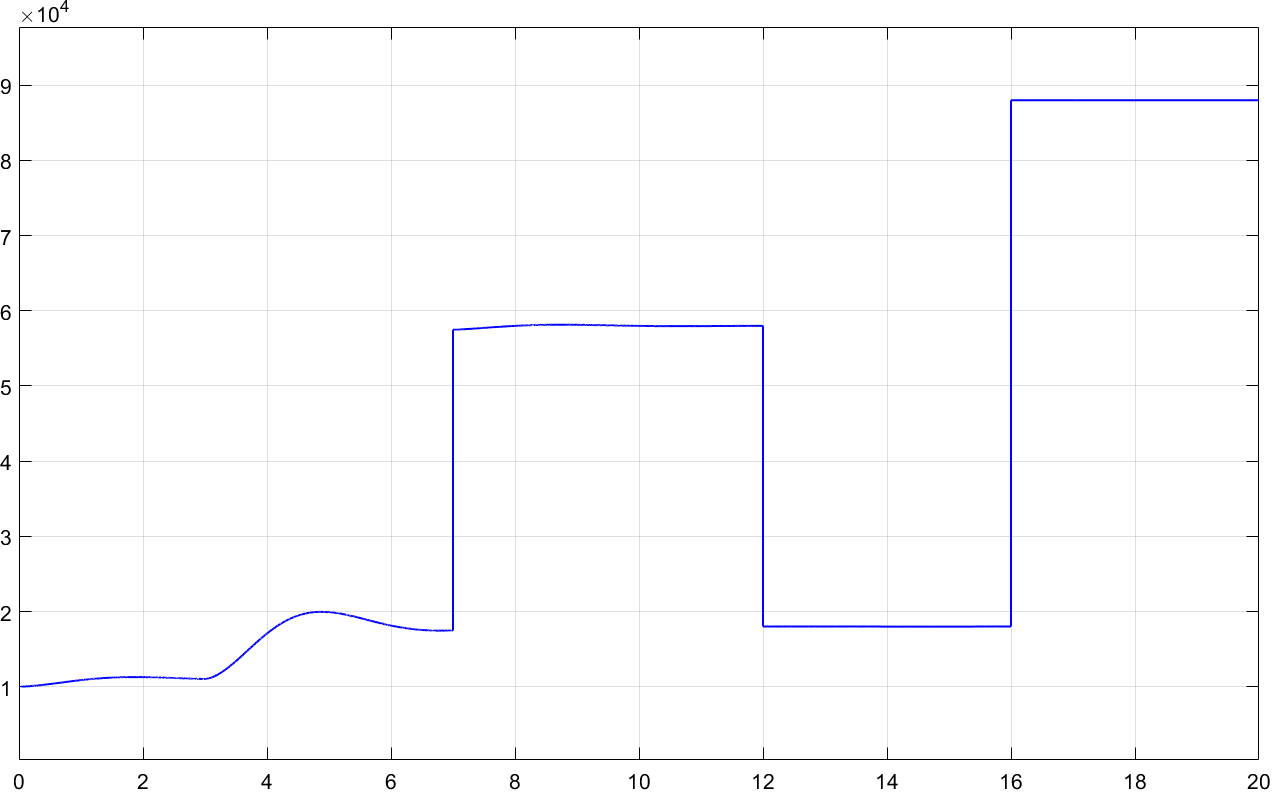
\includegraphics[width=1\textwidth]{rapport/billeder/temporary/load_power}
\caption{Load characteristics for the simulation in power.}
\label{fig:load_power}
\end{figure}

 In \figref{fig:voltage_dist}, the disturbance in the output voltage, caused by the change in load, can be seen.

\begin{figure}[H]
\centering
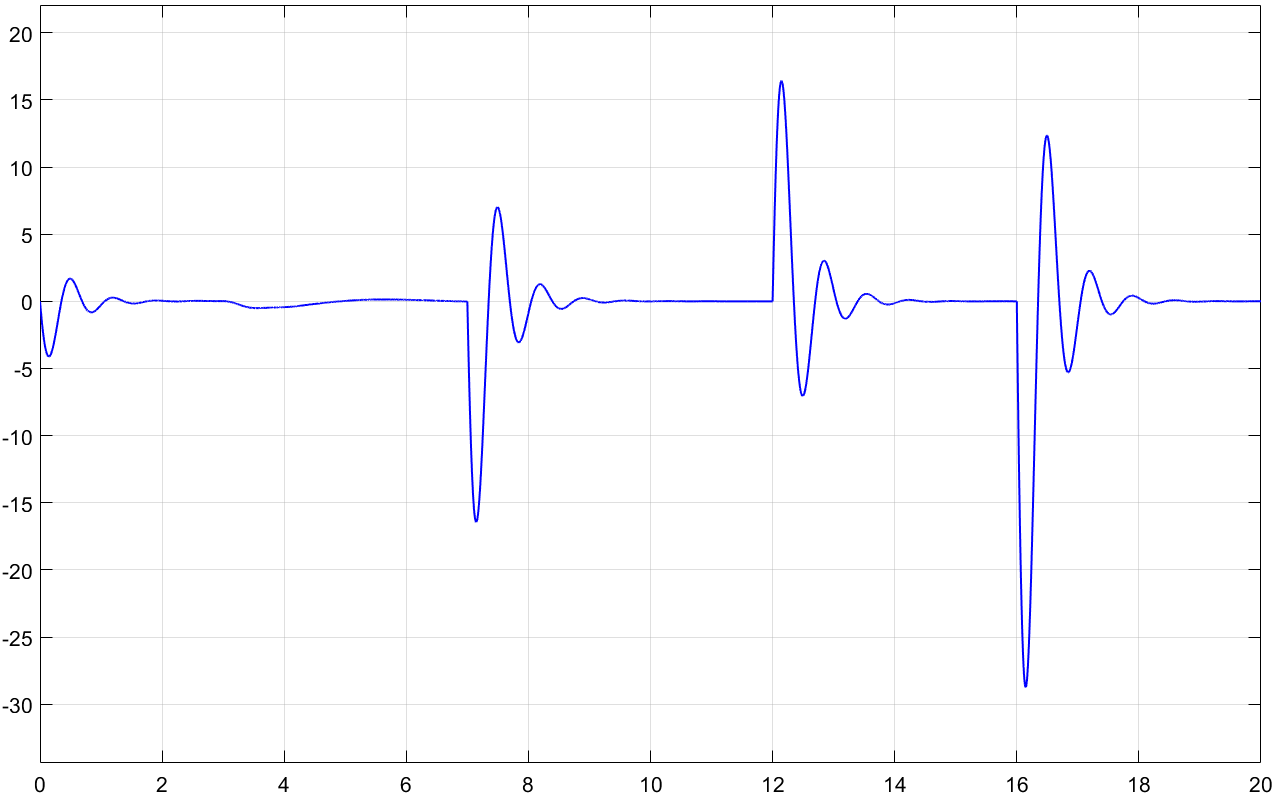
\includegraphics[width=1\textwidth]{rapport/billeder/temporary/load_voltage}
\caption{Voltage disturbance due to changes in the load.}
\label{fig:voltage_dist}
\end{figure}

In \figref{fig:state1} the comparison between the original and the estimated value for the first state can be seen.

\begin{figure}[H]
\centering
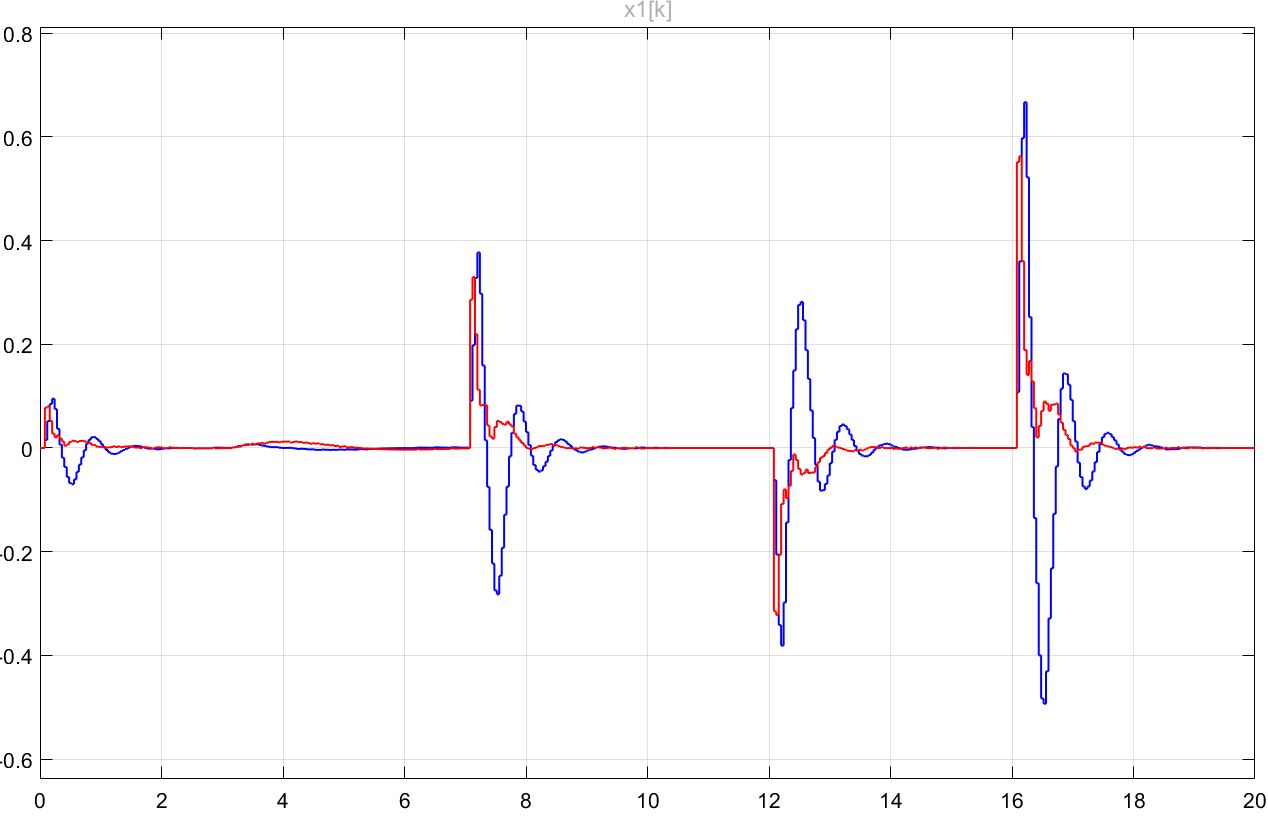
\includegraphics[width=1\textwidth]{rapport/billeder/temporary/state1}
\caption{Comparison of original and estimated value for the first state.}
\label{fig:state1}
\end{figure}

The same comparison for the second state can be seen in \figref{fig:state2}: 

\begin{figure}[H]
\centering
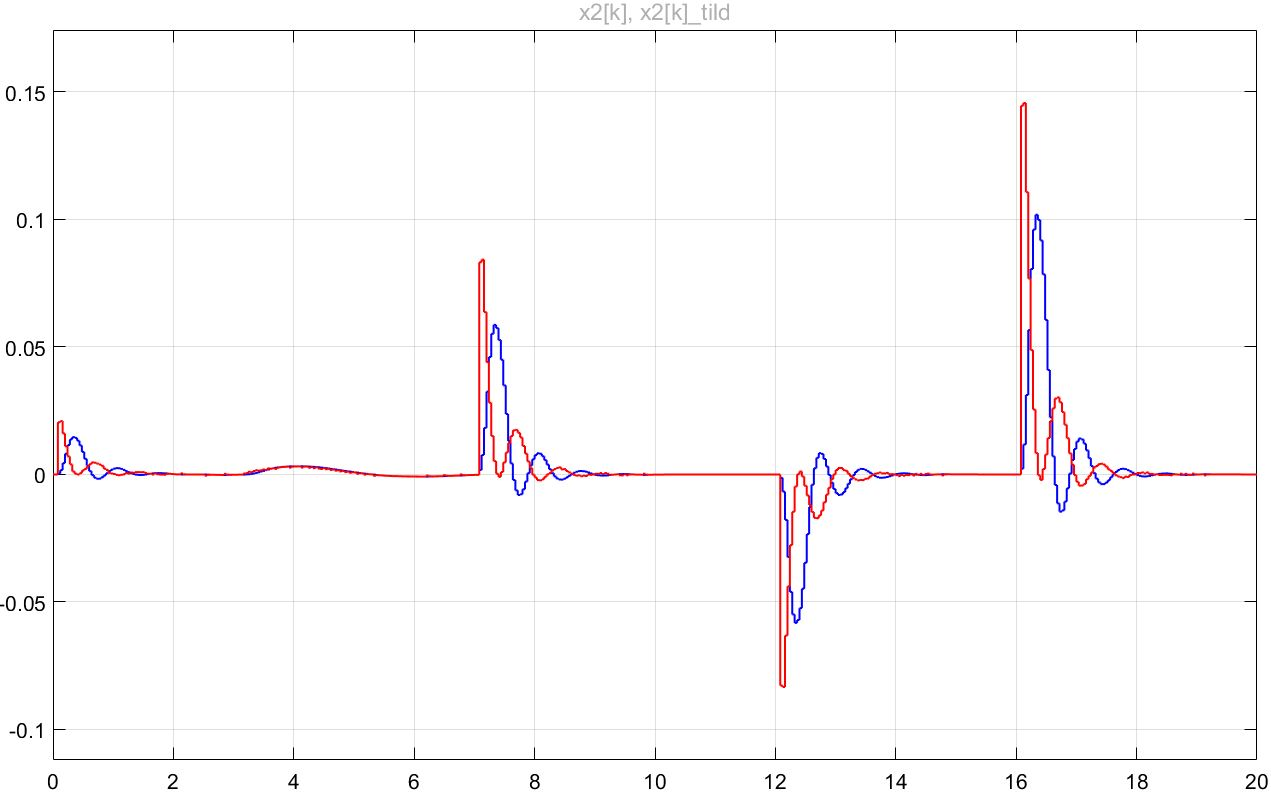
\includegraphics[width=1\textwidth]{rapport/billeder/temporary/state2}
\caption{Comparison of original and estimated value for the second state.}
\label{fig:state2}
\end{figure}

In \figref{fig:errorzero} the size of the error signal is shown.

\begin{figure}[H]
\centering
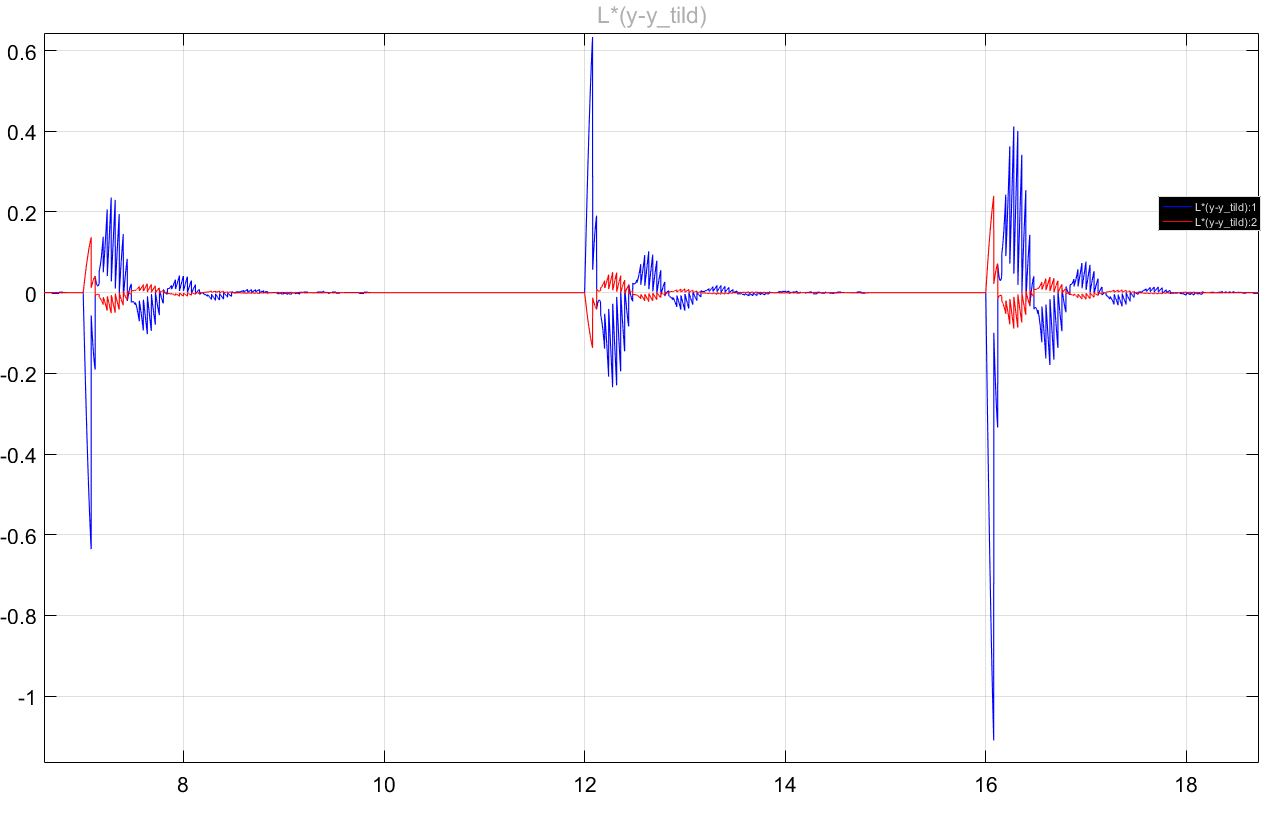
\includegraphics[width=1\textwidth]{rapport/billeder/temporary/errortozero}
\caption{Dynamics of the estimation error.}
\label{fig:errorzero}
\end{figure}

While in \figref{fig:est_out} the estimate of the output is shown. 

\begin{figure}[H]
\centering
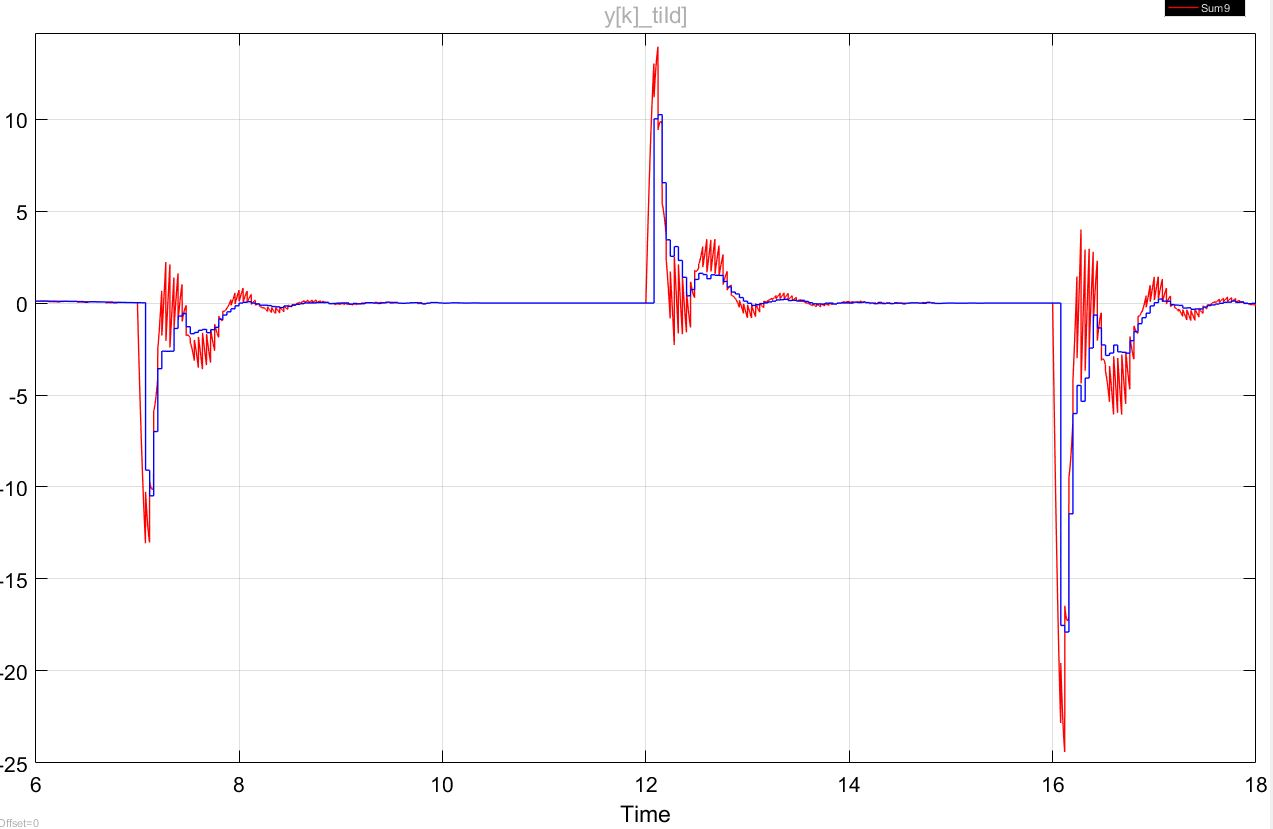
\includegraphics[width=1\textwidth]{rapport/billeder/temporary/outputcomparison}
\caption{Graph showing how the output follows the original output.}
\label{fig:est_out}
\end{figure}